% !TEX root = SocialVision2012.tex

\subsection{Multi-source multi-view network estimation}
\label{sec:vis2net}

In addition to analyzing social interactions in videos, we will investigate tools for analyzing social \emph{relationships}, in terms of the social network that embeds the people observed in an image and video collection. As is customary, we consider the social network of $K$ individuals to be an undirected weighted graph $G$, with $K$ nodes and a non-negative weight ($\in [0,1]$) on the edge between each node-pair. Each  weight represents the social proximity, or strength of tie, between two people, and the weights are collected in a positive symmetric affinity matrix $A$ of size $K\times K$. As described in Sections~\ref{sec:intro} \& \ref{sec:background}, our goal is to develop network reconstruction methods that are well-suited for vision by simultaneously: 1) modeling the multiple-community structure of social networks; 2) incorporating a variety of noisy sources (i.e., social cues automatically extracted from images and videos of varying quality); and 3) tolerating identity errors and high levels of missing data.

It has commonly been observed that social networks include multiple overlapping communities (e.g.,~\cite{AiroldiBFX08,Kim12}). Computationally, this means that the social proximity between nodes is not scalar-valued but depends on the type of roles or memberships (e.g., friends vs. workmates vs. family) by which it is being considered. We refer to these communities as different \emph{views} in the network and we represent them by defining $G\triangleq\{A^{(v)}\}_{v=1}^{V}$, where $A^{(v)}$ is the affinity matrix summarizing the ties between every pair of nodes as measured in the $v$th view. For example, if $v\in\{1,2,3\}$ corresponds to friends, family, and workmates,  $A^{(1)}(i,j)=1$, $A^{(2)}(i,j)=0$, and $A^{(3)}(i,j)=1$ indicates that Alice ($i$) and Bob ($j$) are unrelated but are simultaneously close friends and workmates. 
%The multiple views overlap in general, and the effective tie between each node pair depends on which view is be used to assess their relationship.

In addition to considering multiple views, we will also account for social information coming from multiple distinct cues extracted from visual data, without these cues being associated with peoples' identities with complete certainty. To do this, we consider $S$ \emph{sources} producing socially-informative cues $\vy^s, s=1,2,\cdots,S$, with each $\vy^s(i,j)$ being a multi-dimensional descriptor computed from a distinct socially-informative visual cue related to person $i$ and person $j$. As an example, for a detected, tracked and correctly-identified pair of individuals Alice $(i)$ and Bob $(j)$, a set of sources could include (time-varying in videos): relative positions of the two detections $\vy^1(i,j)$ (or $\vy^1$ for short);  relative head poses $\vy^2$; relative body poses $\vy^3$; distribution over interaction categories $\vy^4$ recovered as in Section~\ref{sec:activity}; and scene category $\vy^5$. These cues will not generally be associated uniquely with one pair of individuals because of uncertainties inherent to face recognition and other forms of identity recognition, and this means that
each source will generally produce from the same image or video sequence multiple differently-weighted outputs. For example, if we cannot visually distinguish Bob ($j$) from Charlie ($k$) then each source will produce from one video sequence two outputs that satisfy $\vy^s(i,j)=\vy^s(i,k)$. 

\boldstart{Restricted regression}. \todd{I just made up this name. Can you think of a better one?} One of our project goals is to establish a unified, data-driven framework for reconstructing multi-view network representations (affinity matrices $A^{(v)}$) from multiple noisy, heterogeneous visual sources. We refer to this problem as multi-source multi-view network estimation, and we will address it using an architecture  comprised of $V$ trained \emph{oracles} $\Psi_{v}$ that each provide an estimate of one view $\hat{A}^{(v)}$ from all available vision-based descriptors $\bar{\vy}=[\vy^1,\vy^2, \cdots,\vy^S]$. That is, $\hat{A}^{(v)}=\Psi_{v}(\bar{\vy})$, with $\Psi_{v}$ learned from data according to the following general approach. Given collections of vision-based social cues $\{\bar{\vy}_{n}\}_{n=1}^{N}$ attributed to $N$ different unknown social network graphs, optionally supplemented by additional collections $\{\bar{\vy}_{n}\}_{n=1}^{M}$ attributed to $M$ graphs that are known (i.e., known 
affinity matrices $\{\bar{A}^{(v)}_{m}\}_{m=1}^{M}$, perhaps through non-visual metadata like that described in Section \ref{sec:sys}), we will investigate a family of objectives of the form
\begin{equation}\label{eq:sensing}
\{\Psi^{*}_{v}\}=\arg\!\!\!\!\!\!\!\!\min_{\{\Psi_{v}\},\{\hat{A}^{(v)}_l\}_{l=1}^{N+M}}\sum_{m=1}^{M}\mathcal{J}\left(\{\Psi_{v}\}, \{\bar{\vy}_m\}, \{\bar{A}^{(v)}_m\}\right)+\tau\left(\{\hat{A}^{(v)}_m\},\{\hat{A}^{(v)}_n\}\right)+\gamma\left(\{\Psi_{v}\}\right).
 \end{equation}
The first term $\mathcal{J}$ in this expression is a loss term that gives preference to oracles that agree with the $M$ known graphs. For example,  $\mathcal{J}(\{\Psi_{v}\}, \{\bar{\vy}_m\}, \{\bar{A}^{(v)}_m\})=\sum_{v=1}^{V}\|\Psi_{v}(\vy_m)-A^{(v)}_m\|^{2}$ would measure discrepancy from the known graphs in a least-squares sense. To prevent over-fitting, the complexity of the oracles is restricted by a regularization term $\gamma()$, whose form depends on the choice of regression machine, such as Gaussian process regression \cite{GPbook} or deep learning \cite{DLbook}. We will also explore modifying this regularization term to enforce compatibility between the oracles of different views. Two oracles predicting friendship and adversarialism for the same pair of nodes, for example, should be deemed incompatible. Finally, we include a third term $\tau()$ that regularizes the estimated affinity matrices according to some generic or environment-specific prior knowledge. For these, we will draw inspiration from the many existing statistical graph models~\cite{Goldenberg}.

In this thread of our research,  cross-view compatibility and within-view clustering are expected to play essential roles in the multi-view architecture. This distinguishes the proposed work from conventional regression machines, where outputs are mutually independent.

%\begin{figure}[t!]
%\begin{center}
%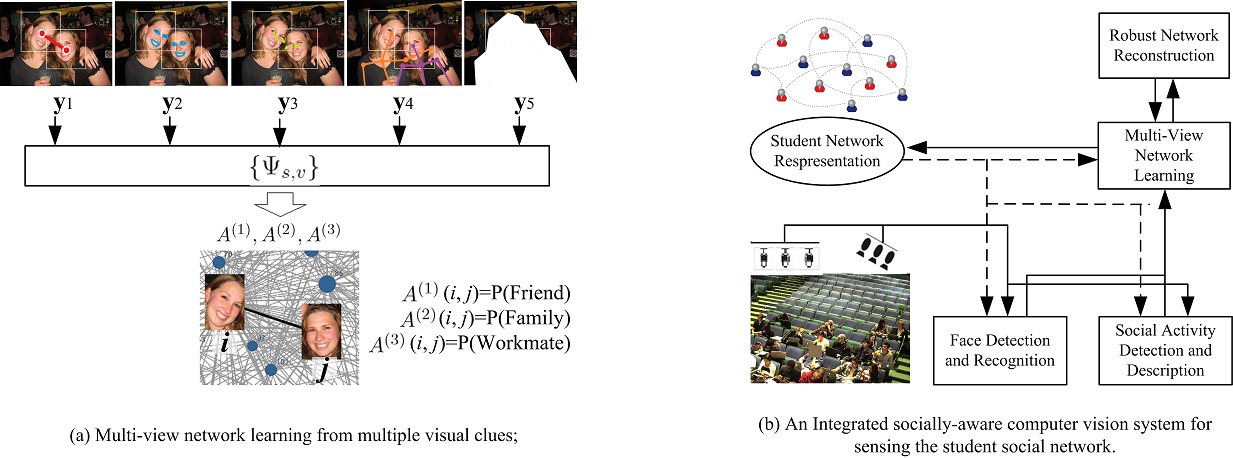
\includegraphics[width=\columnwidth]{featurelearn}
%\end{center}
%\vspace{-0.25in} \caption{\captionsize 
%Illustrations for the problem of multi-view network learning from multiple low-level visual clues and the framework of integrated socially-aware computer vision for understanding student netwrok. \label{fig:featurelearn}\afterfigspace}
%\end{figure}




%%%%%%%%%%%%%%%%%%%%%%%%%%%%%%%%%%%%%%%%%%%%%%%%%%%%%%%%%

%\subsubsection{Associating identities with image targets}
%\label{sec:assoc}

\boldstart{Associating identities with image targets}. To infer a social network from descriptors extracted from detected and tracked agents, we must first associate these vision-based descriptors with the identities of the tracked agents. While face recognition and identity recognition have progressed tremendously during the past decade (see Section~\ref{sec:background}), these systems will continue to suffer from uncertainty well into the future, especially when the input images and videos are low in quality. A key challenge we will address, therefore, is how to succeed in spite of this uncertainty. In doing so we will depart from most existing approaches in network reconstruction (e.g.,~\cite{}\todd{can you add any citations here?}), where even though additive or multiplicative noise might exist in the measured social affinities, these measurements are properly associated with the correct identities/nodes.

One simple approach we will explore is as follows. Suppose we have detected and tracked $L$, and that a face recognition system outputs for each a $K$-dimensional probability histogram $h_l(k)$ describing the likelihood of target $l$ being identity $k$. If facial recognition were perfect, each pair of  tracks would be used to produce one set of visual cues $\vy^s(i,j)$ linked the (certain) identities $i$ and $j$. In the presence of uncertainty, we can enumerate all possible $\prod_{l=0}^{L-1}(K-l)$  assignments, and then (conceptually) duplicate the video $\prod_{l=0}^{L-1}(K-l)$ times considering in each copy that the $L$ targets are assigned according to one of the possible assignments $\{k_1, k_2, \cdots, k_L\}, k_l\in\{1,2, \cdots, K\}$. This produces multiple outputs from each visual source---a descriptor of the form $\vy^s(k_i,k_j)$ for each of the $\prod_{l=0}^{L-1}(K-l)$ conceptual copies. 

The advantage of this approach is that it allows aggregating all of the information available from the recognition system, which we do by ``pooling'' the visual descriptors from all $\prod_{l=0}^{L-1}(K-l)$ copies. We will consider maximum-pooling approaches, $k_l^{*}=\max_{k}h_l(k)$, that select the most probable identity for target $l$ and use only the maximum assignment $\{k_1^{*}, k_2^{*}, \cdots, k_L^{*}\}$ to compute the social cues $\vy^s$ associated with identities $\{k_1^{*}, k_2^{*}, \cdots, k_L^{*}\}$. This strategy essentially assigns each target to a single (possibly incorrect) identity. We will also consider weighted average pooling, where every video copy corresponding to assignment $\{k_1, k_2, \cdots, k_L\}$ contributes to the social cues $\vy^s$ but with a confidence score proportional to the confidence of the recognition system, e.g., $\prod_{l=1}^{L}h_l(k_l)$. In this research, we will not just pursue good empirical results. We will also pursue tractable statistical models for identity uncertainty that can be characterized mathematically, with the goal of creating knowledge that can be more broadly applied to statistical signal processing on graphs and other relational data structures. 